\section{Ρυθμιστής LDO}\label{section:LDO}

Αν και η βασική αρχή λειτουργίας και η απόδοση του LDO παρουσιάστηκαν συνοπτικά στην Ενότητα \ref{section:intro}, η σχεδίαση σε επίπεδο transistor απαιτεί μια βαθύτερη ανάλυση της συμπεριφοράς μικρού σήματος, των παραμέτρων ρύθμισης και της διαστασιολόγησης των εξαρτημάτων. Η παρούσα ενότητα αναλύει τη θεωρητική εξαγωγή των μεγεθών του στοιχείου διέλευσης, την ανάλυση του δικτύου ανάδρασης, παρουσιάζει τα αποτελέσματα των προσομοιώσεων που επιβεβαιώνουν την απόδοση του συστήματος και αναλύει το φυσικό σχέδιο του ρυθμιστή.

% Pass element
\subsection{Διαστασιολόγηση Στοιχείου Διέλευσης ($\symup{M_{pe}}$)}

Για να διασφαλιστεί ότι ο LDO πληροί τις προδιαγραφές $V_{\symup{out}}=0.8\unit{\volt}$ με ρεύμα φορτίου $I_{\symup{load}}=1\unit{\milli\ampere}$ και τάση dropout $V_{sd} \approx 0.4\unit{\volt}$, πρέπει να διαστασιολογηθεί κατάλληλα το pMOS στοιχείο διέλευσης ($\symup{M_{pe}}$) και να αναλυθούν οι παράμετροι κλειστού βρόχου.\par
Το pMOS στοιχείο διέλευσης λειτουργεί στην περιοχή κορεσμού όταν η διαφορά τάσης εισόδου-εξόδου είναι επαρκώς υψηλή ($V_{sd} \gneqq V_{sg} - |V_{th,p}|$), λειτουργώντας ως πηγή ρεύματος ελεγχόμενη από τάση \cite{RazaviFundamentals}. Ωστόσο, σε συνθήκες χαμηλού dropout, ενδέχεται να πλησιάσει την τριοδική περιοχή. Για την παρούσα σχεδίαση, η εξασφάλιση λειτουργίας στον κορεσμό προσφέρει καλύτερη απόρριψη θορύβου τροφοδοσίας. Το ρεύμα που διαρρέει το $\symup{M_{pe}}$ δίνεται από τη σχέση:

\begin{equation}
    I_{d} = \frac{1}{2} \mu_p C_{ox} \left(\frac{W}{L}\right)_{pe} (V_{sg} - |V_{th,p}|)^2 (1 + \lambda V_{sd})
\end{equation}

Αγνοώντας αρχικά τη διαμόρφωση μήκους καναλιού, ο απαιτούμενος λόγος διαστάσεων $S_{\symup{pe}} = (W/L)_{\symup{pe}}$ για την υποστήριξη του μέγιστου ρεύματος φορτίου $I_{\symup{load},\ \max}$ είναι:

\begin{equation}
    S_{\symup{pe}} = \frac{2 I_{\symup{load},\ \max}}{k_{p}^{\prime} \left(V_{sg,\ \max} - |V_{thp}|\right)^2},
\end{equation}
όπου η $V_{sg,\ \max}$ καθορίζεται από την ελάχιστη τάση εξόδου του ενισχυτή σφάλματος \cite{RazaviCMOS}. Με δεδομένες τις παραμέτρους διεργασίας που εκτιμήθηκαν στην Ενότητα \ref{section:EA} ($k_{p}^{\prime} \approx 64.4\unit{\micro\ampere\per\volt\squared}$) και στοχεύοντας σε ελαχιστοποίηση της τάσης υπεροδήγησης (overdrive voltage) για μέγιστο περιθώριο τάσης, υπολογίστηκε το πλάτος $W_{\symup{pe}}$. Η μεγάλη τιμή του $W_{\symup{pe}}$ ελαχιστοποιεί την αντίσταση $R_{\symup{on}}$, αλλά αυξάνει την παρασιτική χωρητικότητα $C_{gd}$, η οποία είναι κρίσιμη για το φαινόμενο Miller που χρησιμοποιείται για την ευστάθεια του συστήματος \cite{Maloberti}.

\subsection{Προσομοιώσεις}

Στην παρούσα υποενότητα αναλύονται τα αποτελέσματα των προσομοιώσεων του κυκλώματος LDO. Οι προδιαγραφές σχεδίασης ορίζουν $V_{\symup{out}} = 0.8\unit{\volt}$ και $I_{\symup{load}} = 1\unit{\milli\ampere}$ με τάση τροφοδοσίας $1.2\unit{\volt}$.

% Pass Element Simulations
\subsubsection{Παραμετρική Ανάλυση: Ρύθμιση του Στοιχείου Διεύλεσης}
Για τον προσδιορισμό των βέλτιστων διαστάσεων του στοιχείου διέλευσης (pass element), διενεργήθηκε παραμετρική ανάλυση (parametric sweep), ελέγχοντας τη συμπεριφορά της τάσης εξόδου υπό συνθήκες μεταβολής της τάσης τροφοδοσίας ($1.2\unit{\volt} \pm 10\%$) και του ρεύματος φορτίου ($1\unit{\milli\ampere} \pm 10\%$), σύμφωνα με τις προδιαγραφές σχεδίασης. Αξιοποιώντας τον σχεδιασμένο ενισχυτή σφάλματος, πραγματοποιήθηκαν προσομοιώσεις στο κύκλωμα \ref{fig:ldo_parametric_analysis} για την επαλήθευση της λειτουργίας σε όλους τους δυνατούς συνδυασμούς γωνιών (corners) λειτουργίας (π.χ. ελάχιστη τάση με μέγιστο φορτίο). Βάσει της σταθερότητας της $V_{\symup{out}}$ σε αυτές τις ακραίες συνθήκες, επιλέχθηκε τελικά πλάτος καναλιού $W = 320\unit{\micro\meter}$. Το μήκος του καναλιού του στοιχείου διέλευσης είναι το μικρότερο δυνατόν, για στοιχεία \texttt{pMOS2v}, $L=150\unit{\nano\meter}$.\par

\begin{figure}[h!]
	\centering
	
\includegraphics[width=0.75\textwidth]{assets/virtuoso/schematics/ldo_real_schematic_v2png.png}
	\caption{Σχηματικό του ρυθμιστή LDO που χρησιμοποιήθηκε για τις προσομοιώσεις εύρεσης μεγέθους του στοιχείου διέλευσης.}
	\label{fig:ldo_parametric_analysis}
\end{figure}

% Line Regulation Simulations
\subsubsection{Ρύθμιση Γραμμής}

Για την αξιολόγηση της ευστάθειας της τάσης εξόδου έναντι μεταβολών της εισόδου, πραγματοποιήθηκε σάρωση της τάσης τροφοδοσίας ($V_{DD}$) στο εύρος $1.08\unit{\volt}$ έως $1.32\unit{\volt}$, το οποίο αντιστοιχεί σε απόκλιση $\pm 10\%$ από την ονομαστική τιμή.

\begin{figure}[h!]
    \centering
    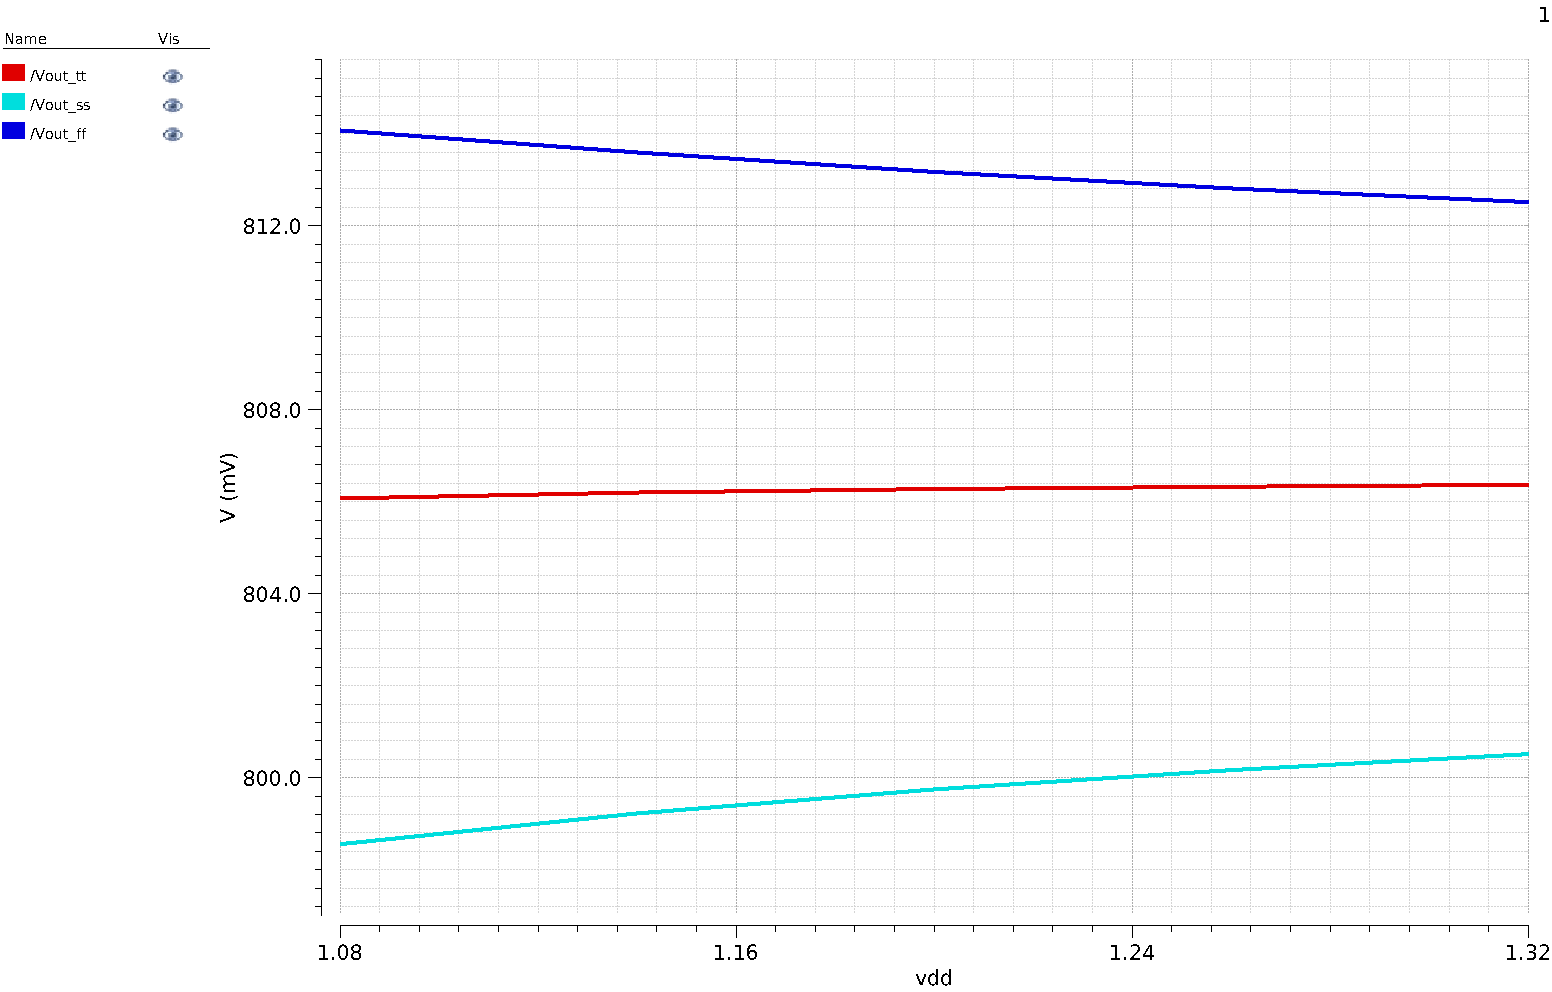
\includegraphics[width=0.8\textwidth]{assets/virtuoso/graphs/vout_vs_vdd.pdf}
    \caption{Διάγραμμα ρύθμισης γραμμής: Μεταβολή της $V_{\symup{out}}$ συναρτήσει της $V_{DD}$ για τις γωνίες TT, FF και SS.}
    \label{fig:line_reg}
\end{figure}

Στο διάγραμμα \ref{fig:line_reg} παρατηρείται ότι η τάση εξόδου παρουσιάζει μια συστηματική απόκλιση μεταξύ των τριών corners (TT, FF, SS), η οποία οφείλεται κυρίως στις μεταβολές της τάσης κατωφλίου $V_{th}$ και της κινητικότητας των φορέων $\mu$ των τρανζίστορ MOSFET. Η γωνία FF (Fast-Fast) εμφανίζει την υψηλότερη τιμή $V_{\symup{out}}$, γεγονός που δικαιολογείται από τη μειωμένη τάση κατωφλίου που αυξάνει το κέρδος και μετατοπίζει το σημείο λειτουργίας της τάσης αναφοράς (Bandgap Reference) προς υψηλότερες τιμές \cite{GrayMeyer}. Αντιστρόφως, η γωνία SS (Slow-Slow) παρουσιάζει τη χαμηλότερη τάση εξόδου, καθώς η αυξημένη $V_{th}$ περιορίζει το διαθέσιμο headroom και μειώνει το ρεύμα ηρεμίας των εσωτερικών σταδίων ενίσχυσης.

Η μορφή των καμπυλών στο διάγραμμα είναι σχεδόν γραμμική με πολύ μικρή κλίση, γεγονός που αποδεικνύει ότι ο βρόχος ανάδρασης λειτουργεί αποτελεσματικά. Η μαθηματική προσέγγιση της ρύθμισης γραμμής ορίζεται ως ο λόγος $\Delta V_{\symup{out}} / \Delta V_{\symup{in}}$ και σχετίζεται άμεσα με το κέρδος ανοικτού βρόχου $A_{ol}$ του ενισχυτή σφάλματος (Error Amplifier). Η ρύθμιση γραμμής βελτιώνεται ανάλογα με το κέρδος του βρόχου, καθώς $V_{\symup{out}} \approx V_{\symup{ref}} \cdot (1 + \nicefrac{R_1}{R_2}) + \nicefrac{V_{DD}}{(A_{ol} \cdot \beta)}$ \cite{BakerJacob}. Η ελαφρώς θετική κλίση που παρατηρείται στις γωνίες TT και SS αποδίδεται στο φαινόμενο διαμόρφωσης μήκους καναλιού (Channel Length Modulation), όπου η αύξηση της $V_{DD}$ οδηγεί σε αύξηση του ρεύματος εξόδου των πηγών ρεύματος, αυξάνοντας ελάχιστα την τάση εξόδου παρά την ανάδραση.

Η αρνητική κλίση που εμφανίζεται στη γωνία FF μπορεί να αιτιολογηθεί από τη μεταβολή του κέρδους του ενισχυτή σφάλματος σε συνάρτηση με την τάση τροφοδοσίας. Σε γρήγορες γωνίες λειτουργίας, η αύξηση της $V_{DD}$ μπορεί να οδηγήσει σε κορεσμό ορισμένων στοιχείων ή σε μεταβολή της συστηματικής απόκλισης (systematic offset) του διαφορικού ζεύγους, προκαλώντας μια ελαφρά υπεραντιστάθμιση από τον βρόχο \cite{MillmanIntegrated}.

Συνολικά, η μικρή απόκλιση μεταξύ των καμπυλών επιβεβαιώνει ότι ο σχεδιασμός είναι αξιόπιστος (robust), καθώς η συνολική μεταβολή παραμένει εντός των προδιαγραφών ανοχής για τυπικά αναλογικά συστήματα σε τεχνολογία CMOS.

% Load Regulation Simulations
\subsubsection{Ρύθμιση Φορτίου}

Η ικανότητα του ρυθμιστή να διατηρεί σταθερή τάση υπό μεταβαλλόμενο φορτίο εξετάστηκε μέσω της σάρωσης του ρεύματος φορτίου ($I_{\symup{load}}$) από $900\unit{\micro\ampere}$ έως $1.1\unit{\milli\ampere}$, καλύπτοντας το εύρος ανοχής $\pm 10\%$.

\begin{figure}[h!]
    \centering
    
\includegraphics[width=0.8\textwidth]{assets/virtuoso/graphs/vout_vs_iload.pdf}
    \caption{Διάγραμμα ρύθμισης φορτίου: Μεταβολή της $V_{\symup{out}}$ συναρτήσει του $I_{\symup{load}}$.}
    \label{fig:load_reg}
\end{figure}

Η ανάλυση του διαγράμματος \ref{fig:load_reg} αποκαλύπτει μια γραμμική πτώση της τάσης εξόδου καθώς αυξάνεται το ρεύμα φορτίου. Η γωνία FF διατηρεί την υψηλότερη τιμή τάσης, άνω των $812\unit{\milli\volt}$, η γωνία TT κυμαίνεται περίπου στα $807\unit{\milli\volt}$, και η γωνία SS εμφανίζει τη χαμηλότερη τιμή, πέφτοντας οριακά κάτω από τα $800\unit{\milli\volt}$ στο μέγιστο φορτίο.\par
Η συμπεριφορά αυτή είναι απόλυτα αναμενόμενη και εξηγείται από τη μη μηδενική αντίσταση εξόδου κλειστού βρόχου ($R_{\symup{out},CL}$) του ρυθμιστή \cite{RazaviCMOS}. Θεωρητικά, η αντίσταση αυτή ισούται με την αντίσταση εξόδου ανοιχτού βρόχου διαιρεμένη με τον παράγοντα $(1 + A\beta)$, όπου $A$ το κέρδος του ενισχυτή και $\beta$ ο συντελεστής ανατροφοδότησης. Η παρατηρούμενη πτώση τάσης επιβεβαιώνει ότι ο LDO λειτουργεί ως πηγή τάσης με χαμηλή, αλλά υπαρκτή, εσωτερική αντίσταση. Η αποτελεσματικότητα της ρύθμισης κρίνεται ικανοποιητική, καθώς η συνολική πτώση τάσης για μεταβολή φορτίου $200\unit{\micro\ampere}$ είναι εξαιρετικά μικρή, υποδεικνύοντας ισχυρό κέρδος βρόχου και σωστή σχεδίαση του ενισχυτή σφάλματος.

% Power Consumption Analysis
\subsection{Κατανάλωση Ισχύος}

\subsubsection{Θεωρητικό Υπόβαθρο και Σημασία}
Η ανάλυση της κατανάλωσης ισχύος είναι κρίσιμη για τη σχεδίαση αναλογικών ολοκληρωμένων κυκλωμάτων, ιδιαίτερα για LDO ρυθμιστές που προορίζονται για φορητές συσκευές τροφοδοτούμενες από μπαταρία (battery-operated devices) \cite{Maloberti}. Σε αυτές τις εφαρμογές, η ενεργειακή αποδοτικότητα καθορίζει άμεσα τη διάρκεια ζωής της συσκευής. Σύμφωνα με τη βιβλιογραφία, η έννοια της ισχύος συνήθως αναφέρεται σε μία από τις εξής κατηγορίες:
\begin{enumerate}
    \item \textbf{Συνολική Ισχύς (Total Power):} Περιλαμβάνει την ισχύ που καταναλώνεται καθόλη τη διάρκεια λειτουργίας του ρυθμιστή.
    \item \textbf{Στατική Ισχύς (Static Power):} Οφείλεται στο ρεύμα ηρεμίας ($I_q$) που ρέει στα εσωτερικά κυκλώματα του LDO (ενισχυτής σφάλματος, διαιρέτες τάσης, κυκλώματα πόλωσης) όταν το φορτίο είναι μηδενικό ή σε κατάσταση αναμονής \cite{Rincón-Mora}. Υπολογίζεται ως $P_{\symup{static}} = V_{\symup{in}} \cdot I_q$.
    \item \textbf{Δυναμική Ισχύς (Dynamic Power):} Περιλαμβάνει την ισχύ που καταναλώνεται κατά των μεταβάσεων (transients) για τη φόρτιση και εκφόρτιση των παρασιτικών χωρητικοτήτων και της χωρητικότητας εξόδου ($P_{\symup{dynamic}} \propto f \cdot C \cdot V^2$) \cite{Rincón-Mora}. Ο υπολογισμός της είναι σύνθετος, μπορεί ωστόσο να οριστεί στην περίπτωσή μας ως η διαφορά της συνολικής με τη στατική ισχύ.

\end{enumerate}

\subsubsection{Μεθοδολογία Προσομοίωσης}
Για την ακριβή μέτρηση των παραπάνω, χρησιμοποιήθηκε η μέθοδος της \textbf{Μεταβατικής Ανάλυσης (Transient Analysis)}, η οποία επιτρέπει τον υπολογισμό της στιγμιαίας ισχύος στον χρόνο \cite{Rincón-Mora}.
Το κύκλωμα τροποποιήθηκε αντικαθιστώντας το σταθερό φορτίο με μια \textbf{Παλμική Πηγή Ρεύματος (Pulse Current Source)}, ώστε να προσομοιωθεί η λειτουργία ενός ψηφιακού φορτίου (π.χ. επεξεργαστή) που εναλλάσσεται μεταξύ κατάστασης «Sleep» και «Active». Χρησιμοποιήθηκε FF corner για τα πιο έντονα αποτελέσματα.

Οι παράμετροι του παλμού ορίστηκαν ως εξής:
\begin{itemize}
    \item \textbf{Low Current (Sleep):} [$0\unit{\ampere}$] (Για μέτρηση στατικής ισχύος).
    \item \textbf{High Current (Active):} [$1\unit{\milli\ampere}$] (Για μέτρηση ισχύος υπό φορτίο).
    \item \textbf{Rise \& Fall Time:} [$10\unit{\nano\second}$] (Για διέγερση δυναμικών φαινομένων).
    \item \textbf{Width:} [$5\unit{\micro\second}$].
\end{itemize}

\begin{figure}[h!]
    \centering
    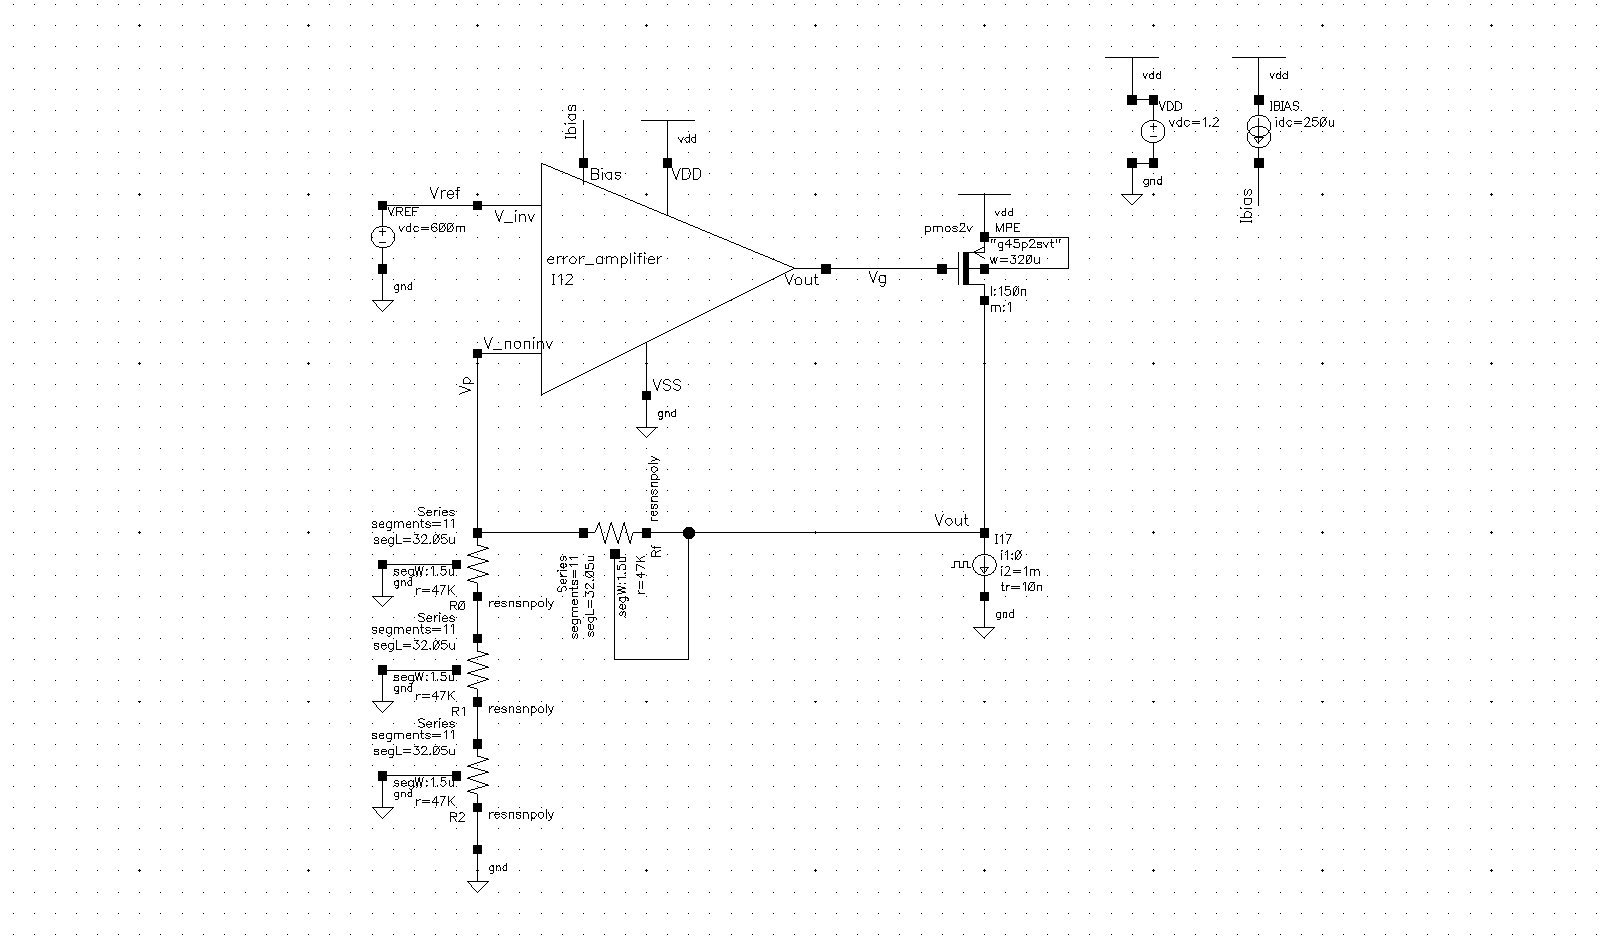
\includegraphics[width=0.7\textwidth]{assets/virtuoso/schematics/testbenches/power_tb.png}
    \caption{Τροποποιημένο σχηματικό για την προσομοίωση ισχύος με χρήση παλμικής πηγής ρεύματος.}
    \label{fig:power_schematic}
\end{figure}

\subsubsection{Ανάλυση Αποτελεσμάτων}
Τα αποτελέσματα της προσομοίωσης απεικονίζονται στο διάγραμμα \ref{fig:power_graph}.

\begin{figure}[h!]
    \centering
    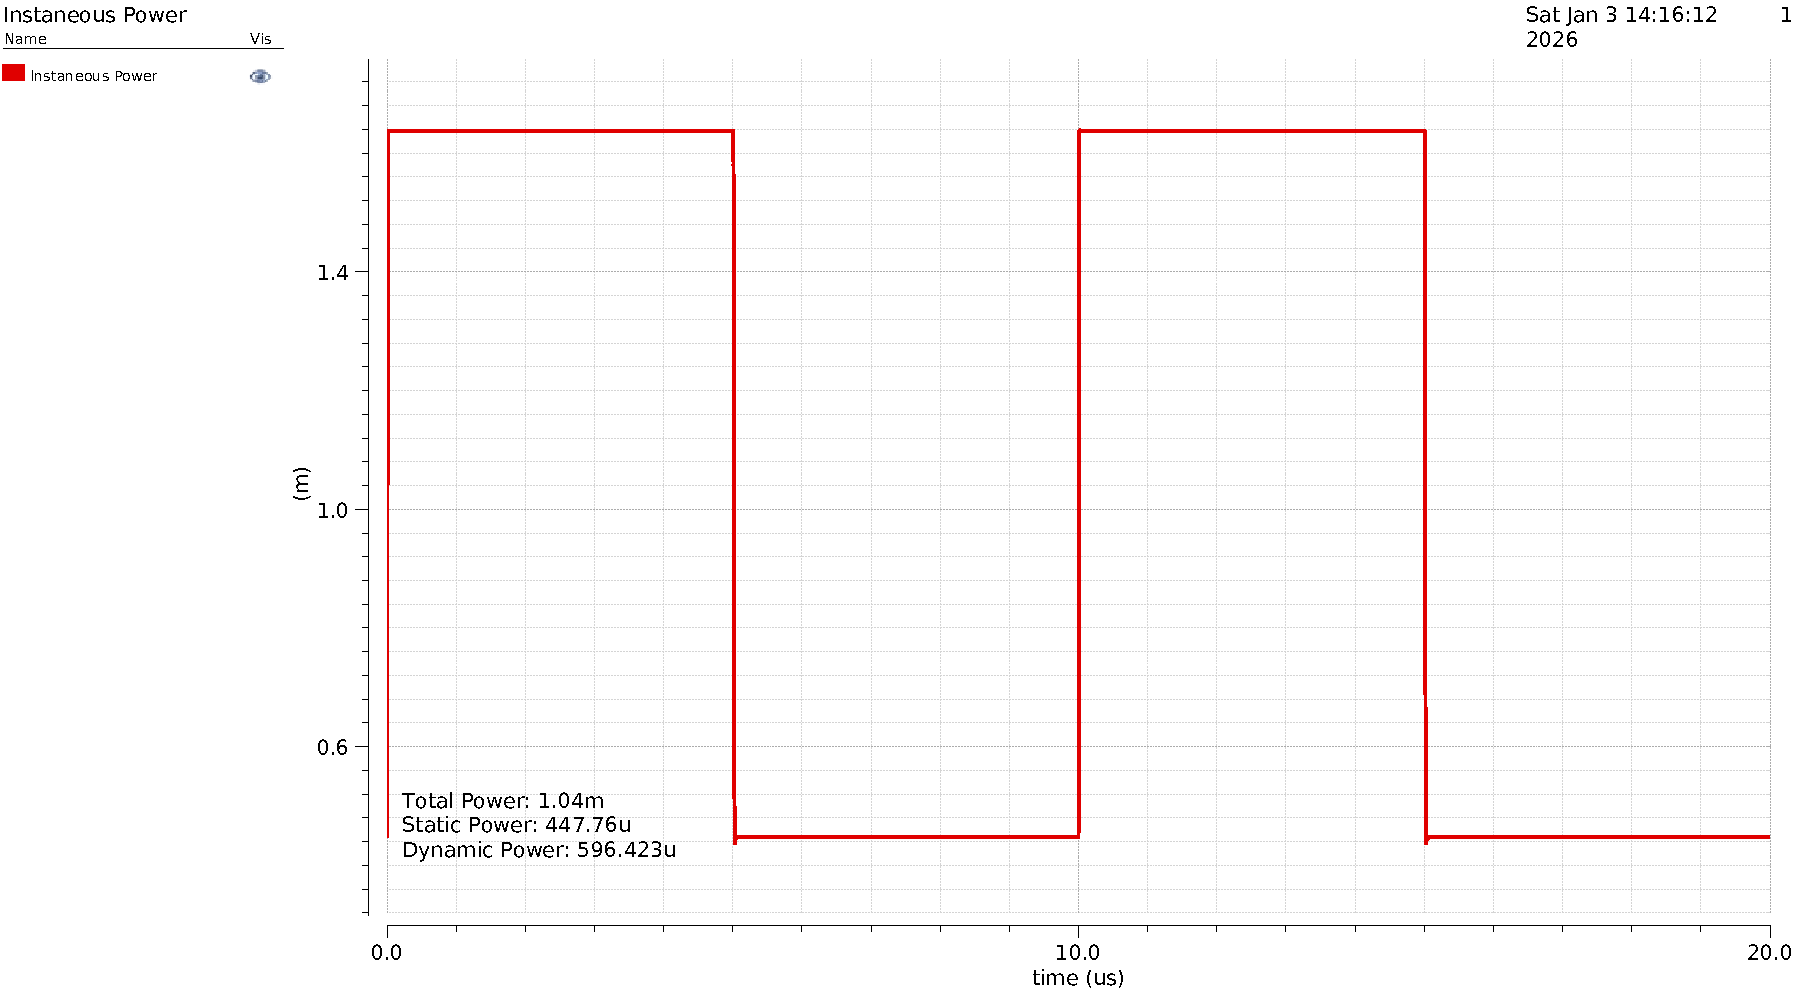
\includegraphics[width=0.8\textwidth]{assets/virtuoso/graphs/LDO_power.pdf}
    \caption{Κυματομορφή στιγμιαίας κατανάλωσης ισχύος. Διακρίνονται οι περιοχές στατικής και ενεργού λειτουργίας.}
    \label{fig:power_graph}
\end{figure}

Όπως φαίνεται στο διάγραμμα \ref{fig:power_graph}, η συνολική μέση κατανάλωση ($P_{\symup{total}}$) υπολογίστηκε στα $1.04\unit{\milli\watt}$. Η τιμή αυτή αναλύεται σε στατική ισχύ $P_{\symup{static}} = 447.76{\unit{\micro\watt}}$, η οποία αντιστοιχεί στο κάτω επίπεδο της κυματομορφής όπου το φορτίο είναι μηδενικό, και σε δυναμική ισχύ $P_{\symup{dynamic}} = 596.423{\unit{\micro\watt}}$, η οποία αντιπροσωπεύει την αύξηση της κατανάλωσης κατά την ενεργοποίηση του φορτίου.

Από πλευράς αποδοτικότητας, αν και η συνολική κατανάλωση παραμένει σε χαμηλά επίπεδα (κοντά στο $1\unit{\milli\watt}$), η στατική ισχύς αποτελεί ένα σημαντικό ποσοστό ($\approx 43\%$) της συνολικής ενέργειας. Αυτό υποδεικνύει ότι, ενώ το κύκλωμα είναι κατάλληλο για εφαρμογές χαμηλής ισχύος, υπάρχει περιθώριο βελτίωσης του ρεύματος ηρεμίας ($I_q$) του ενισχυτή σφάλματος για την περαιτέρω αύξηση της διάρκειας ζωής της μπαταρίας σε καταστάσεις μακράς αναμονής.


% == Physical Layout == %
\subsection{Φυσικό Σχέδιο}

Η παρούσα ενότητα τεκμηριώνει τη φυσική υλοποίηση (layout) του κυκλώματος LDO. Καθώς η ανάλυση της λειτουργίας και η επιλογή των παραμέτρων έχουν παρουσιαστεί σε προηγούμενα στάδια, το ενδιαφέρον εδώ εστιάζεται στη γεωμετρική διάταξη των στοιχείων στο πυρίτιο. Το σχέδιο φαίνεται στην εικόνα \ref{fig:ldo_layout}.

Το τελικό layout επαληθεύτηκε επιτυχώς μέσω των ελέγχων DRC (Design Rule Check) και LVS (Layout Versus Schematic) όπως φαίνεται στο σχήμα \ref{fig:error_amplifier:ldo:layout_DRC_LVS} του παραρτήματος \ref{appendix:layout}, επιβεβαιώνοντας ότι η φυσική υλοποίηση είναι κατασκευαστικά άρτια και πιστή στο ηλεκτρικό σχηματικό, πληρώντας τις προδιαγραφές αξιοπιστίας και απόδοσης που τέθηκαν αρχικά.

\begin{figure}[H]
    \centering
    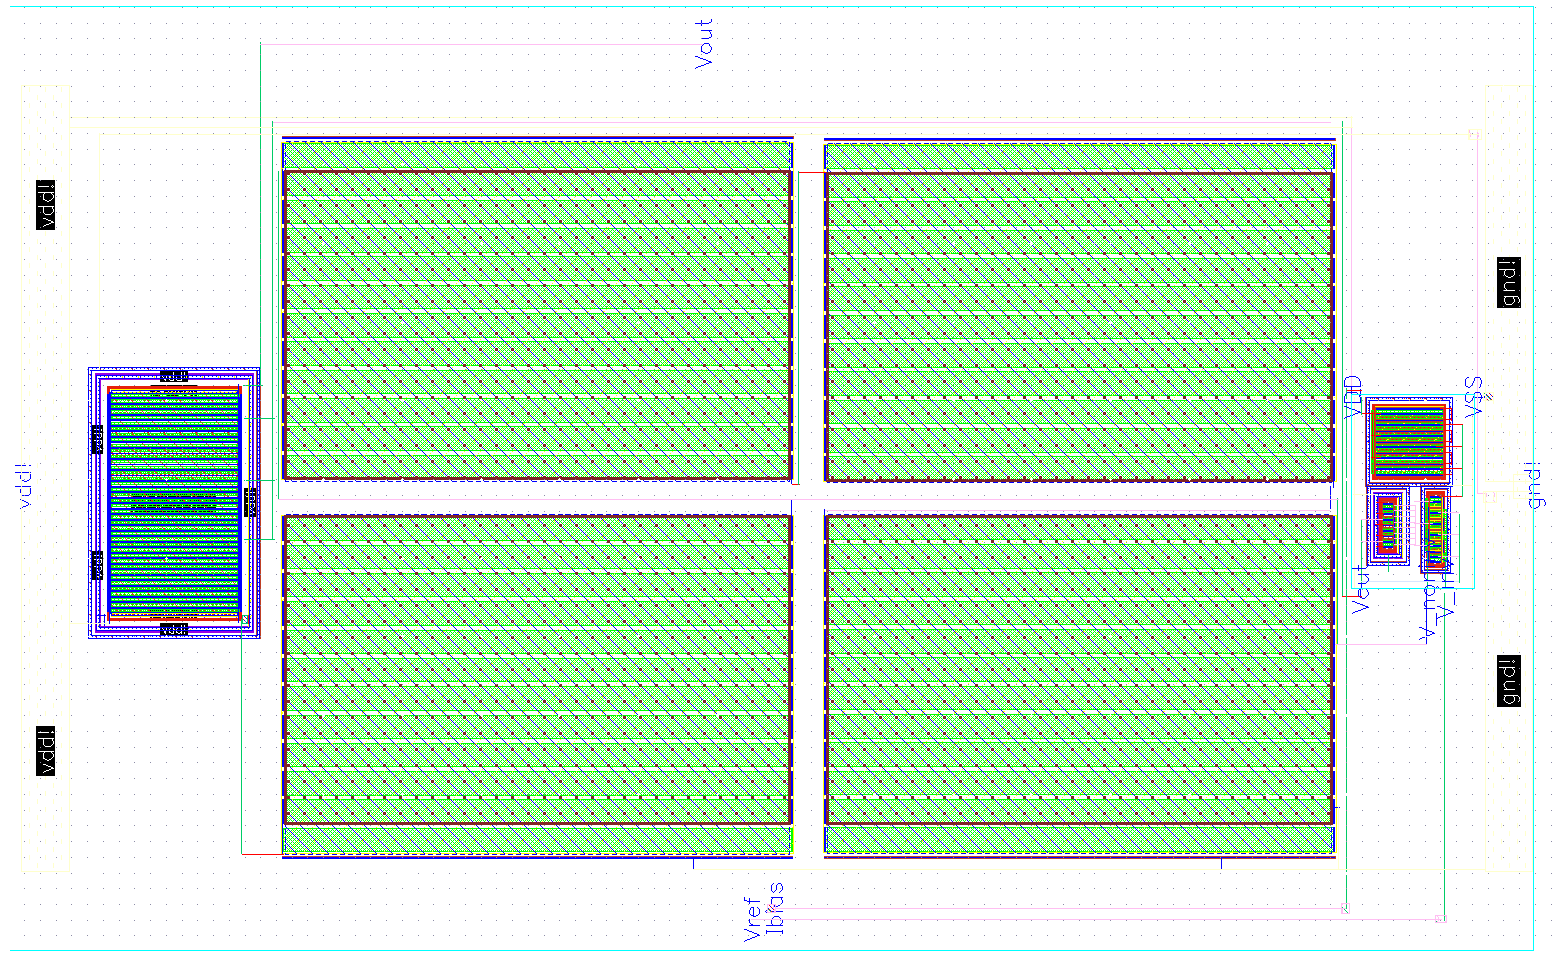
\includegraphics[width=\textwidth]{assets/virtuoso/layout/ldo_flipped_layout.png}
    \caption{Φυσικό σχέδιο του LDO ρυθμιστή. Ακολουθεί η ανάλυση παρακάτω. Στο σχήμα \ref{fig:error_amplifier:ldo:layout_black} το φυσικό σχέδιο παρατίθεται με μαύρο φόντο.}
    \label{fig:ldo_layout}
\end{figure}

% Floorplanning
\subsubsection{Στρατηγική Χωροθέτησης}

Η φυσική σχεδίαση του κυκλώματος υλοποιήθηκε ακολουθώντας μια κάθετη διάταξη στοίβαξης (Vertical Stacking Topology) με τη σειρά: $V_{DD} \rightarrow$ pMOS $\rightarrow$ Αντιστάσεις $\rightarrow$ Ενισχυτής Σφάλματος $\rightarrow$ GND. Η συγκεκριμένη αρχιτεκτονική επιλέχθηκε για τη βελτιστοποίηση της θερμικής συμπεριφοράς και την ακεραιότητα του σήματος.

Το στοιχείο διέλευσης (pMOS) τοποθετήθηκε στο άνω άκρο, σε άμεση επαφή με τη γραμμή τροφοδοσίας ($V_{DD}$), ελαχιστοποιώντας την παρασιτική αντίσταση της πηγής και μεγιστοποιώντας το περιθώριο τάσης (headroom) \cite{BakerJacob}.

Οι αντιστάσεις ανάδρασης τοποθετήθηκαν στο κεντρικό τμήμα της διάταξης, λειτουργώντας ως «θερμικό ανάχωμα» (thermal buffer) που απομονώνει τον ευαίσθητο Ενισχυτή Σφάλματος (κάτω άκρο) από τη θερμότητα που εκλύεται στο pMOS, αποτρέποντας έτσι τη δημιουργία θερμικών κλίσεων στα διαφορικά ζεύγη εισόδου \cite{AlanHasting}.

Για την αντιμετώπιση της μεγάλης απόστασης μεταξύ του ενισχυτή και της πύλης του pMOS, η γραμμή οδήγησης θωρακίστηκε (shielding) ώστε να εξαλειφθεί η χωρητική σύζευξη θορύβου από το δίκτυο αντιστάσεων \cite{RazaviCMOS}.

Η στρατηγική των επαφών (Pin Placement) ακολούθησε γραμμική ροή, με τις ευαίσθητες εισόδους ($V_{\symup{ref}}, I_{\symup{bias}}$) να τοποθετούνται αριστερά και την έξοδο ισχύος ($V_{\symup{out}}$) δεξιά, αποτρέποντας φαινόμενα back-coupling \cite{BakerJacob}.

Τέλος, υιοθετήθηκε τοπολογία αστεροειδούς γείωσης (Star Ground), όπου η γείωση ισχύος και η γείωση σήματος διαχωρίζονται αυστηρά εντός του πυρήνα και ενώνονται μόνο στο σημείο εξόδου, εξαλείφοντας την επίδραση του Ground Bounce στην τάση αναφοράς \cite{GrayMeyer}.


% pMOS Pass Element
\subsubsection{Στοιχείο Διέλευσης}

Λόγω του μεγάλου μεγέθους του pMOS και της έντονης έγχυσης φορέων στο υπόστρωμα, ο κίνδυνος εμφάνισης φαινομένου μανδάλωσης (latch-up) είναι εξαιρετικά αυξημένος. Για την πλήρη εξάλειψη αυτού του κινδύνου, χρησιμοποιήθηκε διπλός δακτύλιος προστασίας (double guard ring) γύρω από το τρανζίστορ. Η διάταξη αυτή αποτελείται από έναν εσωτερικό δακτύλιο επαφών $N^+$ (N-tap ring) συνδεδεμένο στη $V_{DD}$ για τη συλλογή οπών από το N-well, και έναν εξωτερικό δακτύλιο επαφών $P^+$ (substrate ring) συνδεδεμένο στη γείωση ($V_{SS}$) για τη συλλογή ηλεκτρονίων από το υπόστρωμα. Αυτή η διπλή θωράκιση ελαχιστοποιεί τις ωμικές πτώσεις τάσης στο υπόστρωμα και στο well, εμποδίζοντας την ενεργοποίηση της παρασιτικής δομής PNPN \cite{AlanHasting}.

% Feedback Resistors
\subsubsection{Αντιστάσεις Ανάδρασης}
Για την ανάδραση επιλέχθηκαν αντιστάσεις υψηλής ειδικής αντίστασης από πολυπυρίτιο (High-Resistance Poly Resistors), οι οποίες προσφέρουν υψηλή τιμή αντίστασης ανά τετράγωνο (sheet resistance), επιτρέποντας τη μείωση του απαιτούμενου εμβαδού πυριτίου \cite{BakerJacob}.

Οι αντιστάσεις οργανώθηκαν σε μια ενιαία διάταξη συστοιχίας (Resistor Bank) ώστε να εξασφαλιστούν ομοιογενείς θερμικές και κατασκευαστικές συνθήκες. Η ακρίβεια της ρύθμισης του LDO εξαρτάται από το σχετικό ταίριασμα (relative matching) και όχι από την απόλυτη τιμή των αντιστάσεων. Για την ελαχιστοποίηση των σφαλμάτων που προκύπτουν κατά τη διαδικασία της χημικής χάραξης (etching), τοποθετήθηκαν εικονικές αντιστάσεις (dummy resistors) στα δύο άκρα της συστοιχίας. Οι αντιστάσεις αυτές απορροφούν τις αλλοιώσεις που συμβαίνουν στα όρια της μάσκας (boundary effects / etch loading), διασφαλίζοντας ότι οι ενεργές αντιστάσεις στο εσωτερικό της συστοιχίας χαράσσονται ομοιόμορφα και διατηρούν σταθερό πλάτος \cite{AlanHasting}.

Λόγω του μεγάλου μήκους που απαιτείται για την επίτευξη των υψηλών τιμών αντίστασης, υιοθετήθηκε η οφιοειδής γεωμετρική διάταξη (serpentine/snake layout). Η τεχνική αυτή επιτρέπει την αναδίπλωση του υλικού σε συμπαγή ορθογώνια δομή, βελτιστοποιώντας τη χρήση του διαθέσιμου χώρου χωρίς να επηρεάζεται η συνολική τιμή της αντίστασης \cite{RazaviCMOS}.


% Vias
\subsubsection{Σχεδίαση Επαφών}

Οι κάθετες διασυνδέσεις μεταξύ των μεταλλικών επιπέδων (vias) αποτελούν συχνά σημεία αστοχίας λόγω της συγκέντρωσης ρεύματος (current crowding). Η χρήση μεμονωμένων vias αποφεύχθηκε συστηματικά στις γραμμές ισχύος, καθώς αυξάνουν την παρασιτική αντίσταση και αποτελούν μονοσήμαντα σημεία αποτυχίας (single points of failure). Αντ' αυτού, υιοθετήθηκε η χρήση συστοιχιών επαφών (via arrays / redundant vias). Η τεχνική αυτή διαμοιράζει το ρεύμα σε πολλαπλά παράλληλα μονοπάτια, μειώνοντας δραστικά την αντίσταση επαφής και διασφαλίζοντας τη λειτουργία του κυκλώματος ακόμα και σε περίπτωση κακής κατασκευής ενός μεμονωμένου via \cite{AlanHasting}. Το πλήθος των επαφών επιλέχθηκε έτσι ώστε να μπορεί να διέλθει ρεύμα μεγαλύτερο του προσομοιωμένου.\par

% Antenna Effect
\subsubsection{Φαινόμενο Κεραίας}
Κατά το στάδιο της φυσικής σχεδίασης, δόθηκε ιδιαίτερη βαρύτητα στη θωράκιση των πυλών των τρανζίστορ έναντι του φαινομένου της κεραίας (Antenna Effect). Το φαινόμενο αυτό εκδηλώνεται κατά τη διαδικασία της χάραξης πλάσματος (plasma etching), όπου οι αγωγοί μεγάλου μήκους που συνδέονται αποκλειστικά στην πύλη ενός MOS τρανζίστορ συμπεριφέρονται ως κεραίες, συλλέγοντας φορτία ιόντων. Εάν η συσσώρευση φορτίου υπερβεί ένα κρίσιμο όριο, το επαγόμενο δυναμικό δύναται να προκαλέσει μη αναστρέψιμη διάσπαση του οξειδίου της πύλης ($t_{ox}$ breakdown) ή, εναλλακτικά, να υποβαθμίσει μακροπρόθεσμα την αξιοπιστία της διάταξης μέσω της έγχυσης θερμών φορέων \cite{AlanHasting}.

Για τη συμμόρφωση με τους κανόνες σχεδίασης (Antenna DRC Rules), εξετάστηκε η γραμμή ελέγχου του pMOS ισχύος ($V_g$), η οποία χαρακτηρίζεται από εκτεταμένο μήκος διασύνδεσης. Παρότι η αυξημένη επιφάνεια του αγωγού συνεπάγεται υψηλό κίνδυνο συλλογής φορτίου, δεν απαιτήθηκε η εφαρμογή τεχνικών διακοπής μέσω αλμάτων (jumper breaking). Η επιλογή αυτή τεκμηριώνεται από το γεγονός ότι ο κόμβος οδηγείται απευθείας από τη διάχυση (drain diffusion) της εξόδου του ενισχυτή σφάλματος. Σύμφωνα με τη βιβλιογραφία, η ύπαρξη αγώγιμης διάχυσης συνδεδεμένης στον κόμβο δημιουργεί μια δίοδο προστασίας ως προς το υπόστρωμα. Κατά τη διάρκεια της κατασκευής, η εν λόγω δίοδος λειτουργεί ως ασφαλής δίοδος εκφόρτισης, καθώς είτε πολώνεται ορθά είτε οδηγείται σε ελεγχόμενη κατάρρευση χιονοστιβάδας (avalanche breakdown). Μέσω αυτού του μηχανισμού, το αναπτυσσόμενο δυναμικό ψαλιδίζεται (clamping) σε επίπεδα ασφαλή για την ακεραιότητα του οξειδίου της πύλης, καθιστώντας περιττή την προσθήκη επιπλέον στοιχείων προστασίας \cite{AlanHasting}.